\documentclass[11pt]{article}
\usepackage[utf8]{inputenc}
\usepackage[english]{babel}
\usepackage{amsmath}
\usepackage{graphicx}
\usepackage{float}
\usepackage{lipsum}
\usepackage{multicol}
\usepackage{xcolor}
\usepackage{tabularx}
\usepackage{booktabs}
\usepackage{hyperref}
\newcolumntype{Y}{>{\centering\arraybackslash}X}
\usepackage[left=2.00cm, right=2.00cm, top=2.00cm, bottom=2.00cm]{geometry}
\usepackage{enumitem}

\title{AN2DL Reports Template}

\begin{document}

\begin{figure}[H]
      \raggedright
      
\includegraphics[scale=0.4]{polimi.png} \hfill
      
\includegraphics[scale=0.3]{airlab.jpeg}
\end{figure}

\vspace{5mm}

\begin{center}
      % Select between First and Second
      {\Large \textbf{AN2DL - Second Homework Report}}\\
      \vspace{2mm}
      % Change with your Team Name
      {\Large \textbf{LosPollosHermanos}}\\
      \vspace{2mm}
      % Team Members Information
      {\large Mohammadhossein Allahakbari,}
      {\large Michele Miotti,}
      {\large Francesco Pesce}\\
      \vspace{2mm}
      % Codabench Nicknames
      {mh2033,}
      {michelem,}
      {francescopesce}\\
      \vspace{2mm}
      % Matriculation Numbers
      {246639,}
      {249499,}
      {247974}\\
      \vspace{5mm}
      \today
\end{center}
\vspace{5mm}

\begin{multicols}{2}
      % Note: The following sections represent a suggested
      % structure. We don't need to follow it strictly.

      % -----------------------------------------------------------------------
      % INTRODUCTION
      % -----------------------------------------------------------------------
      \section{Introduction}
      % In this section, you should present your project's context and
      % objectives. You might want to:
      % \begin{itemize}
      %     \item Dehe problem (\textit{you may use italics to highlight
      %               definitions})
      %     \item State your goals (\textbf{emphasise key points with bold})
      %     \item Outline your approach
      % \end{itemize}

      % \noindent For instance, you might write: ``This project focuses on
      % \textit{image classification} using \textbf{deep learning} techniques."

      This report presents the results of the \textit{semantic segmentation}\cite{long2015fullyconvolutionalnetworkssemantic}
      task proposed in the second homework of the \texttt{Artificial Neural Networks and Deep Learning} course. Its goal is to classify each pixel in $64\times128$ grayscale images of the Mars surface in one of $5$ classes, each representing a different type of terrain or object: background, soil, bedrock, sand or big rock, similarly to \cite{li2024marssegmarssurfacesemantic}.

      % -----------------------------------------------------------------------
      % PROBLEM ANALYSIS
      % -----------------------------------------------------------------------
      \section{Problem Analysis}
      \label{sec:analysis}
      % Here you can discuss your initial analysis of the problem. Consider
      % including:
      % \begin{enumerate}
      %     % 8 classes, 96x96 rgb images, labels, etc
      %     \item Dataset characteristics
      %     \item Main challenges % The test set is horrible
      %     That the test set was not horrible? Is this what they mean?
      %     \item Initial assumptions 
      % \end{enumerate}

      % \noindent If you need to reference papers, use the citation command:
      % Recent work~\cite{lecun2015deep} suggests..."

      We were provided two separate datasets, containing around $2500$ and $10000$ images respectively, which we modelled as generated by the same distribution. The former contained \textit{labeled} images, and was used to train the model, while the latter was unlabeled, and was instead used to evaluate our models, by uploading the models' predictions to the \texttt{Kaggle}\cite{kaggle} platform. This last dataset was further split into two subsets, the first of which containing about $25\%$ of the data, used to provide public evaluations during the competition, while the other subset contained the rest of the data, and was used for the final evaluation. The three datasets will be reffered to as \texttt{DS1}, \texttt{DS2} and \texttt{DS3} respectively. After manually analyzing \texttt{DS1}, we found and discarded $110$ images doctored with unraled \textit{overlays}. Moreover, analyzing its labels, we found them to be rather imprecise, as they were labelled by hand. This lack of precision can be modelled as a contribution of a \textit{bias} in the labelling process, caused by the same type of imprecisions being repeated in a consistent way, and of an added \textit{variability} of the dataset. We found no need to relabel the images in \texttt{DS1}, as a rich model should be capable of learning the bias of the labelling process, while the added variability in \texttt{DS3} cannot be removed by any process.

      Given an image segmentation model, for each class $i$, we define $A_i$ as the set of labels belonging to class $i$ and $B_i$ as the set of labels the model classifies as belonging to class $i$. The \textit{Intersection over Union}(IoU) metric for class $i$ is defined as: $$\text{IoU}_i = \dfrac{|A_i \cap B_i|}{|A_i \cup B_i|}$$ and models are evaluated based on the \textit{Mean IoU} metric, defined as the mean of the IoU metrics over all non-background classses.

      % -----------------------------------------------------------------------   
      % METHOD
      % -----------------------------------------------------------------------
      \section{Method}
      % Not sure what they are asking here. The final model?
      % This section should detail your approach. You can use equations to
      % explain your methodology. For example, a simple model representation:
      % \begin{equation}
      %     \label{eq:model}
      %     f(x) = \text{softmax}(Wx + b)
      % \end{equation}

      % \noindent Or a more complex loss function:
      % \begin{equation}
      %     \label{eq:loss}
      %     \mathcal{L} = -\frac{1}{N}\sum_{i=1}^{N} y_i\log(\hat{y}_i)
      % \end{equation}

      % \noindent Reference these equations in your text, like:``As shown in
      % equation~\ref{eq:model}..."

      Most of the development process employs \texttt{Jupyter} notebooks, using the \texttt{Tensorflow}\cite{TensorFlow} and \texttt{Keras}\cite{chollet2015keras} libraries for \texttt{Python}. Except for very early models, which were trained on \texttt{Google Colab}, and the last few models, which were trained on \texttt{Kaggle} due to hardware limitations, training was performed locally using an \texttt{NVIDIA RTX 2060 Mobile}.

      In order to validate the model, we split the training set into a training and \textit{validation} set, containing between $10\%$ and $20\%$ of the data depending on the model. Differently from the first homework, we noticed that the validation and \texttt{DS2} MIoUs were similar, so we were able to avoid submitting models with low validation MIoU.

      All models we produced share the same basic structure, displayed in Figure \ref{fig:model_structure}. It is heavily inspired by the U-Net\cite{ronneberger2015unetconvolutionalnetworksbiomedical} architecture, capable of capturing both \textit{local information} and the \textit{global context}. The \textit{contracting path} is composed of a series of $k$ convolutional and downsampling layers, where each layer halves the spatial dimensions of the input, while doubling the number of channels. The \textit{expanding path} is composed of a series of convolutional and up-sampling layers, which act as the opposite of the previous layers, doubling the spatial dimensions and halving the number of channels. 

      \begin{figure}[H]
            \centering
            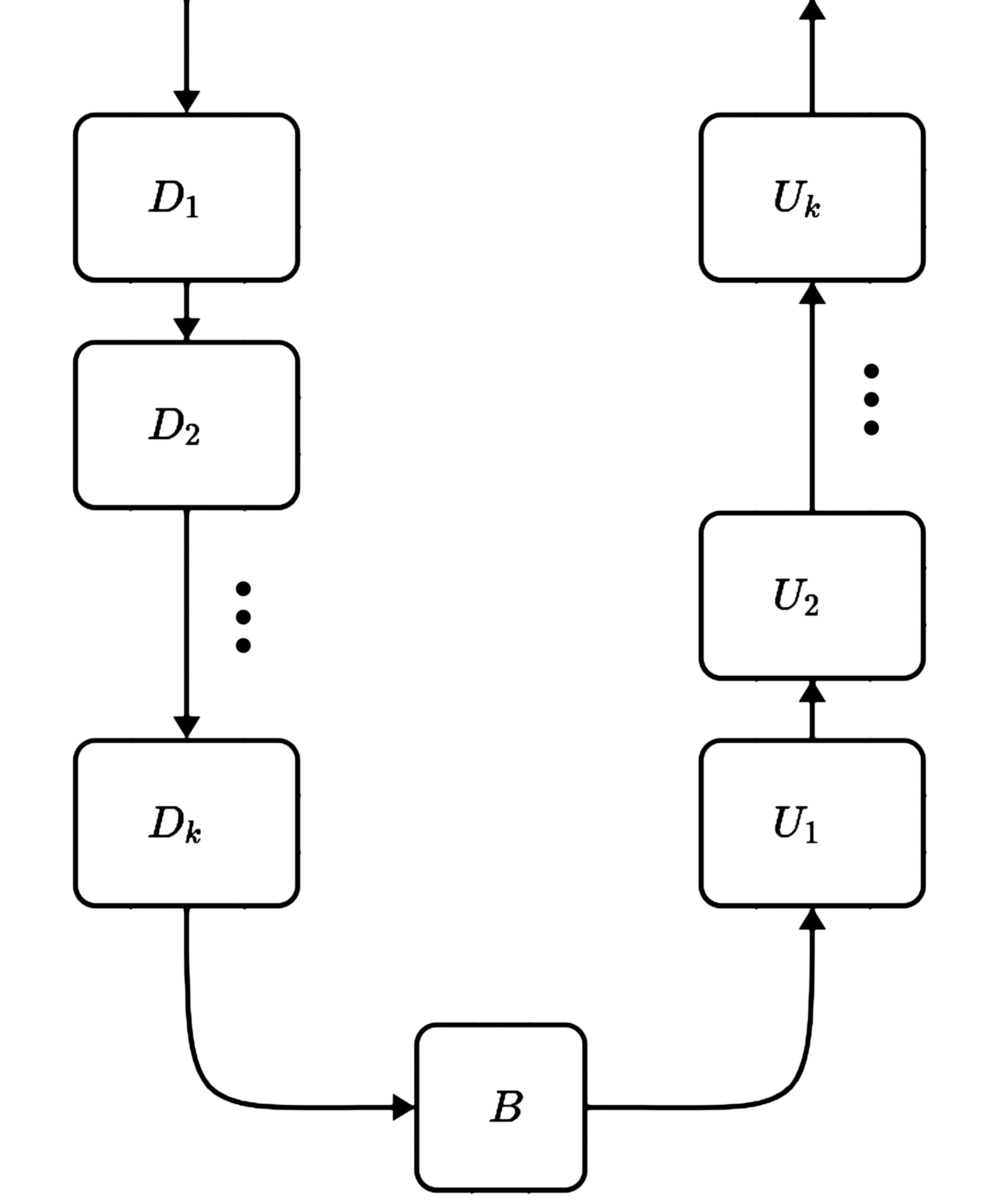
\includegraphics[width=0.7\linewidth]{model-structure.png}
            \caption{The basic structure of our models, shown here with $k$ layers. On the left, the contracting path, known as the \texttt{Encoder}, in the middle, the \texttt{Bottleneck}, and on the right the expanding path, known as the \texttt{Decoder}, are displayed.}
            \label{fig:model_structure}
      \end{figure}

      % -----------------------------------------------------------------------
      % EXPERIMENTS
      % -----------------------------------------------------------------------
      \section{Experiments}
      \label{sec:experiments}
      During development, we tested around $100$ different models, with our experiments being broadly categorizable in 4 categories:
      \begin{itemize}[leftmargin=*]
            \setlength\itemsep{0em}
            \item \textbf{Initial experiments:} We started development using a simple U-Net-like architecture with 3 layers, to get a baseline of the model's performance, and then introduced simple image \textit{augmentations} such as flips, zooms and changes in brightness to increase the model's robustness. Spatial augmentations were also applied to the labels, so that they'd refer to the transformed version of their own pixel. Our first obstacle was the model's inability to learn consistently, as minor changes to the model or even the seed would result in the training processes halting at a MIoU of less then $0.1$. The issue was likely the fact that the training process remained stuck in a \textit{local minimum}, and the more \textit{noisy gradient estimations} produced by a lower \textit{batch size} were able to solve the problem, allowing us to use larger networks.
            \item \textbf{Model M1:} By following our experience with the first homework, we replaced $3\times3$ convolutions with our custom block (described in detail in the previous report), which is formed by a stack of \texttt{Inception} blocks followed by residual connections. Moreover, to directly optimize the model for the evaluation, we decided to implement a loss function based on the MIoU, by directly accessing the backend from \texttt{Keras}. Since it needs to be \textit{differentiable}, it is computed using the posterior probabilities outputted by the model instead of just their maximum, and its sign is flipped to use \textit{gradient descent}. Finally, we inserted \texttt{Attention Gates}\cite{oktay2018attentionunetlearninglook}, which are connections between contracting and expanding paths of the same size, so that he model is able to focus on the most important parts of the image, and carefully analyzed the complex \textit{design space} for model architecture and hyperparameters. These changes resulted in a model with $1.8$ million parameters, and a MIoU on \texttt{DS2} of $0.595$, trained using \texttt{AdamW} with initial learning rate $1e-4$, adaptively lowered during training.
            \item \textbf{Failed experiments:} To try and improve M1's architecture, we performed many failed experiments, requiring by far the most development time. These experiments include replacing $5\times5$ convolutions with $3\times3$ \textit{dilated} convolutions to mantain the large \textit{receptive field} while reducing the number of parameters, inserting a \texttt{Transformer}\cite{vaswani2023attentionneed} block in the bottleneck layer, using augmentations provided by the KerasCV library, taking care to only use augmentations which preserve \textit{local statistics}, and using different optimizers. We considered adding a second \textit{classification head} classifying the outputs of the intermediate layer of the contracting path, trained using downsampled versions of the labels, and using its MIoU in the loss function, to incentivise the lower level to learn the desired features, while keeping a baseline performance for the upper level, experimenting with many weighting techniques, including adaptive ones. We also tried inserting the predictions M1 to the inputs of a separate model, training the latter with inputs in the form \textit{(image, prior\_prediction)}, with skip connections between M1 predictions and the outputs, with the rationale that this could work as a sort of residual architecture, but without the need for more memory during training. Finally, we experimented with separate models for background and big rock recognition, as discussed in Section \ref{sec:conclusions}.
            \item \textbf{Model M2:} Model M2 differs from prior models in two key aspects: it uses simpler $3\times3$ convolutions in each layer instead of stacking our custom block multiple times, and the number of layers in the contracting and expanding paths is 5 instead of 2, with upsampling being beformed using \textit{fractional stride} convolutions. This architecture has around $99$ million parameters and is more prone to overfitting, prompting the addition of \texttt{Spatial Dropout} layers, \textit{L2 normalization} in convolutions and change from \texttt{Batch Normalization} to \texttt{Group Normalization} layers. Since the architecture no longer benefits from the presence of \texttt{Attention Gates}, they were removed, and a \texttt{Focal}\cite{lin2018focallossdenseobject} loss term, weighted with inverse class frequencies excluding the background, was added to the global loss, with a weight of $0.2$. The higher number of layers and parameters was capable of capturing more of the images' features, resulting in a higher MIoU of $0.629$ on \texttt{DS2}.
      \end{itemize}

      % For your experiments, you might want to present your results in tables.
      % Here's an example of a wide table comparing different models:

      % \begin{table*}[t]
      %     \centering
      %     \setlength{\tabcolsep}{3pt}
      %     \caption{An example of wide table. Best results are highlighted in
      %         \textbf{bold}.}
      %     \begin{tabularx}{\textwidth}{lYYYc}
      %         \toprule
      %         Model            & Accuracy                  & Precision
      %                          & Recall                    & ROC AUC
      %         \\
      %         \midrule
      %         VGG18            & 72.20 $\pm$ 3.06          & 94.95 $\pm$ 0.52
      %                          &
      %         86.95 $\pm$ 0.55 & 80.16 $\pm$ 0.81
      %         \\
      %         Custom Model     & 27.71 $\pm$ 3.19          & 75.70 $\pm$ 1.07
      %                          & 55.75 $\pm$ 2.16          & 36.60 $\pm$ 1.26
      %         \\
      %         ResNet18         & \textbf{89.24 $\pm$ 2.38} & \textbf{95.54
      %         $\pm$ 0.49}      & \textbf{93.43 $\pm$ 1.30} & \textbf{91.68 $\pm$
      %             0.71}
      %         \\
      %         \bottomrule
      %     \end{tabularx}
      %     \label{tab:Performance}
      % \end{table*}

      % \noindent For more specific measurements, you might use a narrower
      % table:

      % \begin{table}[H]
      %     \centering
      %     \setlength{\tabcolsep}{3pt}
      %     \caption{An example of table. Best results may be highlighted in
      %         \textbf{bold}.}
      %     \begin{tabularx}{\linewidth}{lY}
      %         \toprule
      %         Time [$\mu$s] & Distance [mm] \\
      %         \midrule
      %         22$\pm$4      & 8$\pm$1       \\
      %         17$\pm$3      & 7$\pm$1       \\
      %         15$\pm$3      & 6$\pm$1       \\
      %         13$\pm$2      & 5$\pm$1       \\
      %         10$\pm$2      & 4$\pm$1       \\
      %         8$\pm$2       & 3$\pm$1       \\
      %         5$\pm$1       & 2$\pm$1       \\
      %         37$\pm$1      & 1$\pm$1       \\
      %         \bottomrule
      %     \end{tabularx}
      %     \label{tb:Measurements}
      % \end{table}

      % \noindent You can also include figures to visualise your results:
      % \begin{figure}[H]
      %     \centering
      %     
\includegraphics[width=0.75\linewidth]{random.jpeg}
      %     \caption{Example figure showing [describe what the figure shows]}
      %     \label{fig:results}
      % \end{figure}

      % \noindent Reference figures using like:``As shown in
      % Figure~\ref{fig:results}..."

      % -----------------------------------------------------------------------
      % RESULTS
      % -----------------------------------------------------------------------
      \label{sec:results}
      \section{Results}
      % Present your main findings here. You might want to:
      % \begin{itemize}
      %     \item Compare your results with baselines
      %     \item Highlight key achievements using \textbf{bold text}
      %     \item Explain any unexpected outcomes
      % \end{itemize}

      \begin{table}[H]
            \label{tab:results}
            \centering
            \setlength{\tabcolsep}{3pt}
            \begin{tabularx}{\linewidth}{lY}
                \toprule
                Experiment & Mean IoU \\
                \midrule
                Simple U-Net & 0.38328 \\
                Augmentation & 0.44328 \\
                Batch size reduction & 0.45797 \\
                Custom block & 0.45911 \\
                IoU loss & 0.48808 \\
                Attention gates (M1) & 0.59533 \\
                Deeper architectures (M2) & 0.62900 \\
                \bottomrule
            \end{tabularx}
      \end{table}

      Table \ref{tab:results} displays the highest MIoU on \texttt{DS2} using the succesful techniques discussed in Section \ref{sec:experiments}, before introducing the next technique. For each technique, multiple models were tested, and the highest result is reported in the table.

      % -----------------------------------------------------------------------
      % DISCUSSION
      % -----------------------------------------------------------------------
      \section{Discussion}
      % In this section, analyse your results critically. Consider:
      % \begin{itemize}
      %     \item Strengths and weaknesses
      %     \item Limitations and assumptions
      % \end{itemize}

      We developed a deep and robust image segmentation network, capable of performing image segmentation of Mars terrain images, despite the issues of the labeling process described in Section \ref{sec:analysis}. Analyzing the \textit{confusion matrix} on the validation set, it appears the model captures well the features of three terrain types, with a MIoU on said terrains of over $0.8$. The largest weaknesses of the model is the fact that it performs poorly on the big rock class, as it was not capable of learning the class's features from just the $63$ images in \texttt{DS1} that feature the class. A further weaknesses of M2 is that it is not trainable on commodity hardware, and cannot even be used for prediction on devices with lower capabilities. In this regard, we propose the usage of model M1, which has a slightly lower MIoU, but solves the previously mentioned issue, as it was trained on mid-range laptop GPU from several generations ago.

      % -----------------------------------------------------------------------
      % CONTRIBUTIONS
      % -----------------------------------------------------------------------
      \section{Contributions}

      Most ideas and propositions were evenly distributed among the team members, while actual coding was more specific to each member's strengths. The final model and many of the failed experiments are the result of discussing potential improvements and ides between team members.

      % -----------------------------------------------------------------------
      % CONCLUSIONS
      % -----------------------------------------------------------------------
      \section{Conclusions}
      \label{sec:conclusions}
      % Summarise your work and discuss potential future directions. This is
      % where you can:
      % \begin{itemize}
      %     \item Restate main contributions
      %     \item Suggest improvements
      %     \item Propose future work
      % \end{itemize}

      In this challenge, we were able to tackle an \textit{image segmentation} task and develop close to $100$ models, exploring the design space of \textit{image segmentation} architectures, with our final model obtaining a MIoU on non-background classes of $0.629$ on \texttt{DS2}. Future work centers around the poor performance of our models on the big rock class, as they often misclassifies the background as a big rock. An idea we would like to further explore is developing separate models for big rock or background recognition. While we experimented with both, considering both the options of using the full dataset and just the images containing big rocks, obtaining no meaninful results, we believe that the idea has potential, especially if coupled with a technique to generate more big rock samples, either using a larger dataset or with advanced image augmentation techniques. Since the current IoU for the class is close to 0, even a small improvement would hugely impact the final MIoU of the model.

      % Remember to include the bibliography!
      \bibliography{references}
      \bibliographystyle{abbrv}

\end{multicols}
\end{document}